\documentclass[xetex]{beamer}
\usepackage{kotex}
\usetheme{Copenhagen}
\usepackage{fontspec}
\usepackage{xunicode}
\usepackage{xltxtra}
\usepackage{unicode-math}
\usefonttheme{serif}
\setmainfont{NanumGothicBold}
\setmathfont[range=\mathup/{num}]{NanumGothicBold}
\setmathfont[range={"00D7}]{NanumGothicBold}
\begin{document}
\title{2017 서울대학교 프로그래밍 경시대회}
\date{\today}

\frame{\titlepage}

\begin{frame}
  \frametitle{수고하셨습니다}
  \begin{itemize}
    \item 총 참가자 45명
    \item 총 제출 횟수: 931
    \item 총 정답 횟수: 182
    \item 참고로 문제 배치는 랜덤입니다.
  \end{itemize}
\end{frame}

\begin{frame}
  \frametitle{Div2A. 여우 사인}
  \begin{itemize}
    \item 제출 횟수: ??
    \item 맞은 참가자 수: ??
    \item 정답률: ??\%
    \item 처음 맞은 참가자: ??
    \item 출제자: 임동재
  \end{itemize}
\end{frame}

\begin{frame}
  \frametitle{Div2A. 여우 사인}
  \begin{itemize}
    \item 여우는 사랑입니다.
    \item 입력이 정확히 $(1, 3)$, $(1, 4)$, $(3, 4)$ 세 개의 쌍으로만 이루어져 있는지 판별하면 됩니다.
  \end{itemize}
\end{frame}

\begin{frame}
  \frametitle{Div2B. 고장난 시계}
  \begin{itemize}
    \item 제출 횟수: ??
    \item 맞은 참가자 수: ??
    \item 정답률: ??\%
    \item 처음 맞은 참가자: ??
    \item 출제자: 박상언
  \end{itemize}
\end{frame}

\begin{frame}
  \frametitle{Div2B. 고장난 시계}
  \begin{itemize}
    \item 판이 크지는 않아요.
    \item 반드시 전구가 배치되어야 하는 곳과 그렇지 않은 곳이 있어요.
    \item 나머지는 잘 채워나가면 돼요.
  \end{itemize}
\end{frame}

\begin{frame}
  \frametitle{Div2C. 타일 뒤집기 (Easy)}
  \begin{itemize}
    \item 제출 횟수: ??
    \item 맞은 참가자 수: ??
    \item 정답률: ??\%
    \item 처음 맞은 참가자: ??
    \item 출제자: 임동재
  \end{itemize}
\end{frame}

\begin{frame}
  \frametitle{Div2C. 타일 뒤집기 (Easy)}
  \begin{itemize}
    \item 어떤 타일의 바로 위나 같은 행의 타일을 뒤집을 수 없을 때, 그 타일을 뒤집으려면 반드시 바로 아래 타일을 뒤집어야 합니다.
    \item 첫 행부터 답이 되는 타일을 뒤집고, 현재 상태와 답을 비교해서 다음 행에서 뒤집어야 할 타일을 구하면 됩니다.
  \end{itemize}
\end{frame}

\begin{frame}
  \frametitle{Div2D \& Div1B. 관악산 등산}
  \begin{itemize}
    \item 제출 횟수: ??
    \item 맞은 참가자 수: ??
    \item 정답률: ??\%
    \item 처음 맞은 참가자: ??
    \item 출제자: 임동재
  \end{itemize}
\end{frame}

\begin{frame}
  \frametitle{Div2D \& Div1B. 관악산 등산}
  \begin{itemize}
    \item Corea가 가는 경로는 항상 높이가 증가하는 순입니다.
    \item $cnt_{i} = \max_{H[j] > H[i]} cnt_{j} + 1$
    \item 높은 곳에 있는 쉼터부터 $cnt$를 결정하면 됩니다.
  \end{itemize}
\end{frame}

\begin{frame}
  \frametitle{Div2E. 넴모넴모 (Easy)}
  \begin{itemize}
    \item 제출 횟수: ??
    \item 맞은 참가자 수: ??
    \item 정답률: ??\%
    \item 처음 맞은 참가자: ??
    \item 출제자: 임동재
  \end{itemize}
\end{frame}

\begin{frame}
  \frametitle{Div2E. 넴모넴모 (Easy)}
  \begin{itemize}
    \item $N \times M$이 작으므로 모든 배치를 탐색하면 됩니다.
    \item 깊이 우선 탐색 등을 이용해 배치할 수 없을 때마다 커팅하는 것을 의도했습니다.
    \item 일단 배치를 만들고 가능한지 검사하는 방식으로는 시간 내에 들기 힘듭니다.
  \end{itemize}
\end{frame}

\begin{frame}
  \frametitle{Div2F. 앵무새}
  \begin{itemize}
    \item 제출 횟수: ??
    \item 맞은 참가자 수: ??
    \item 정답률: ??\%
    \item 처음 맞은 참가자: ??
    \item 출제자: 오평석
  \end{itemize}
\end{frame}

\begin{frame}
  \frametitle{Div2F. 앵무새}
  \begin{itemize}
    \item 답은 $100,000$ 이하로 나와요.
    \item 모든 가능한 분모에 대해 분자를 구하고, 그 결과가 입력과 같은지를 확인하면 돼요.
  \end{itemize}
\end{frame}

\begin{frame}
  \frametitle{Div2G \& Div1D. 셔틀버스}
  \begin{itemize}
    \item 제출 횟수: ??
    \item 맞은 참가자 수: ??
    \item 정답률: ??\%
    \item 처음 맞은 참가자: ??
    \item 출제자: 임동재
  \end{itemize}
\end{frame}

\begin{frame}
  \frametitle{Div2G \& Div1D. 셔틀버스}
  \begin{itemize}
    \item 왼쪽 절반은 항상 왼쪽으로, 오른쪽 절반은 항상 오른쪽으로 이동합니다.
    \item 양쪽의 학생 수를 알면 주어진 자리가 비어 있는지, 혹은 몇 번째로 번호가 작은 학생이 앉아 있는지 구할 수 있습니다.
    \item 구간 트리 등의 자료구조를 사용하면 학생이 내리는 연산과 $k$번째 학생을 구하는 연산을 빠르게 처리할 수 있습니다.
    \item $N$이 홀수일 때 가운데에 앉은 학생은 맨 처음 내리는 학생의 위치에 따라 이동 방향이 달라집니다.
  \end{itemize}
\end{frame}

\begin{frame}
  \frametitle{Div2H. 홍삼 게임 (Easy)}
  \begin{itemize}
    \item 제출 횟수: ??
    \item 맞은 참가자 수: ??
    \item 정답률: ??\%
    \item 처음 맞은 참가자: ??
    \item 출제자: 임동재
  \end{itemize}
\end{frame}

\begin{frame}
  \frametitle{Div2H. 홍삼 게임 (Easy)}
  \begin{itemize}
    \item 각 지목권이 어떤 사람에게 있는지, 어떤 지목권이 사용될 차례인지를 알고 있으면 게임의 상태를 나타낼 수 있습니다.
    \item 총 $2 \times N^{2}$개의 상태에 대해 너비 우선 탐색 등의 방법으로 두 지목권이 겹칠 때까지의 최단거리를 구하면 됩니다.
    \item 어떤 지목권이 사용될 차례인지를 최단거리의 홀짝성으로 판별하면 틀립니다.
  \end{itemize}
\end{frame}

\begin{frame}
  \frametitle{Div2I. 전생했더니 슬라임 연구자였던 건에 대하여 (Easy)}
  \begin{itemize}
    \item 제출 횟수: ??
    \item 맞은 참가자 수: ??
    \item 정답률: ??\%
    \item 처음 맞은 참가자: ??
    \item 출제자: 박성원
  \end{itemize}
\end{frame}

\begin{frame}
  \frametitle{Div2I. 전생했더니 슬라임 연구자였던 건에 대하여 (Easy)}
  \begin{columns}
    \column{0.65\textwidth}
      \begin{itemize}
        \item 슬라임을 분해하는 과정을 오른쪽과 같이 이진트리로 모델링 할 수 있습니다.
        \item 단말노드의 개수는 소인수의 개수와 같습니다.
      \end{itemize}
    \column{0.35\textwidth}
      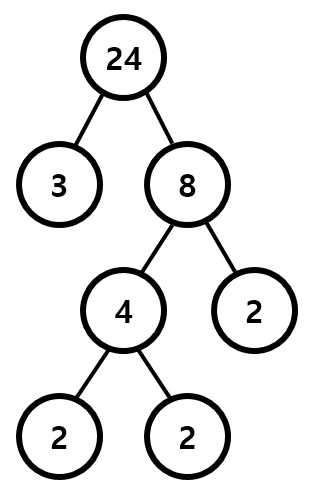
\includegraphics[width=1\textwidth]{slime-sol-0.png}
  \end{columns}
\end{frame}

\begin{frame}
  \frametitle{Div2I. 전생했더니 슬라임 연구자였던 건에 대하여 (Easy)}
  \begin{columns}
    \column{0.5\textwidth}
      \begin{itemize}
        \item 전체 높이를 최소로 만들려면 각 분할과정마다 단말노드가 절반으로 나눠지도록 하면 됩니다.
        \item $N = p_1^{q_1} p_2^{q_2} ...$ 라면 답은 $\lceil \log_2(p_1 + p_2 + ...) \rceil$
        \item 수의 범위가 작으니 DP로 접근할 수도 있습니다.
      \end{itemize}
    \column{0.5\textwidth}
      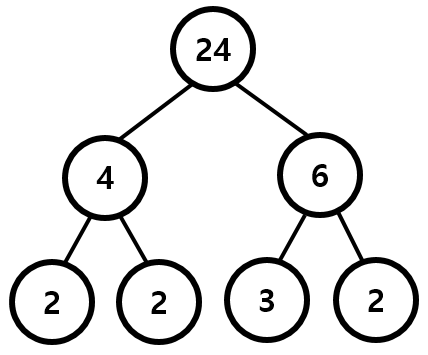
\includegraphics[width=0.9\textwidth]{slime-sol-1.png}
  \end{columns}
\end{frame}

\begin{frame}
  \frametitle{Div1A. 전생했더니 슬라임 연구자였던 건에 대하여 (Hard)}
  \begin{itemize}
    \item 제출 횟수: ??
    \item 맞은 참가자 수: ??
    \item 정답률: ??\%
    \item 처음 맞은 참가자: ??
    \item 출제자: 박성원
  \end{itemize}
\end{frame}

\begin{frame}
  \frametitle{Div1A. 전생했더니 슬라임 연구자였던 건에 대하여 (Hard)}
  \begin{columns}
    \column{0.65\textwidth}
      \begin{itemize}
        \item Easy 와는 반대로, 단말노드가 주어졌을 때 비용이 최소가 되는 이진트리를 구성하는 문제입니다.
        \item 총 비용 $C$는 각 단계의 비용 $A \times B$ 들의 곱입니다.
        \item $\log(C)$는 $\log(A) + \log(B)$ 들의 합입니다.
      \end{itemize}
    \column{0.35\textwidth}
      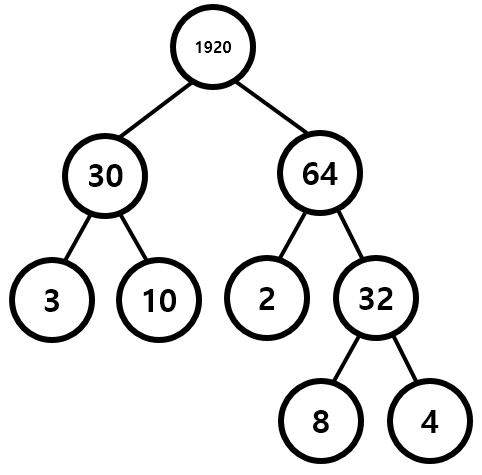
\includegraphics[width=1\textwidth]{slime2-sol-0.png}
  \end{columns}
\end{frame}

\begin{frame}
  \frametitle{Div1A. 전생했더니 슬라임 연구자였던 건에 대하여 (Hard)}
  \begin{itemize}
    \item $\log(c_i)$ 를 갖고 허프만 트리를 만들면 전체 비용이 최소가 됩니다.
  \end{itemize}
\end{frame}

\begin{frame}
  \frametitle{Div1C. 넴모넴모 (Hard)}
  \begin{itemize}
    \item 제출 횟수: ??
    \item 맞은 참가자 수: ??
    \item 정답률: ??\%
    \item 처음 맞은 참가자: ??
    \item 출제자: 임동재
  \end{itemize}
\end{frame}

\begin{frame}
  \frametitle{Div1C. 넴모넴모 (Hard)}
  \begin{itemize}
    \item 어떤 칸에 넴모를 배치할 수 있는지 확인하려면 그 칸의 왼쪽, 위, 왼쪽 위 칸의 정보가 필요합니다.
    \item 따라서 어떤 칸의 이전 $N + 1$개 칸의 정보만 알고 있으면 충분합니다.
    \item Bitmask DP로 해결 가능합니다.
  \end{itemize}
\end{frame}

\begin{frame}
  \frametitle{Div1E. 데굴데굴}
  \begin{itemize}
    \item 제출 횟수: ??
    \item 맞은 참가자 수: ??
    \item 정답률: ??\%
    \item 처음 맞은 참가자: ??
    \item 출제자: 임동재
  \end{itemize}
\end{frame}

\begin{frame}
  \frametitle{Div1E. 데굴데굴}
  \begin{itemize}
    \item 수면이 덮는 점은 연속된 구간입니다.
    \item Two pointers 테크닉으로 구간을 잘 관리하면서 변의 개수를 잘 세면 됩니다.
    \item 물이 물병을 꽉 채우는 경우 등 주의할 경우가 조금 있습니다.
  \end{itemize}
\end{frame}

\begin{frame}
  \frametitle{Div1F. 전자기기}
  \begin{itemize}
    \item 제출 횟수: ??
    \item 맞은 참가자 수: ??
    \item 정답률: ??\%
    \item 처음 맞은 참가자: ??
    \item 출제자: 윤지학
  \end{itemize}
\end{frame}

\begin{frame}
  \frametitle{Div1F. 전자기기}
  \begin{itemize}
    \item 문제를 풀기 위해 아래 지식이 필요해요.
    \begin{itemize}
      \item 2차원에서 직사각형 영역의 부분합을 빠르게 구하는 방법 (cf. BOJ 11660)
      \item 주어진 히스토그램에서 가장 큰 직사각형의 넓이를 구하는 방법 (cf. BOJ 1725)
      \item 포함배제의 원리
    \end{itemize}
  \end{itemize}
\end{frame}

\begin{frame}
  \frametitle{Div1G. 타일 뒤집기 (Hard)}
  \begin{itemize}
    \item 제출 횟수: ??
    \item 맞은 참가자 수: ??
    \item 정답률: ??\%
    \item 처음 맞은 참가자: ??
    \item 출제자: 임동재
  \end{itemize}
\end{frame}

\begin{frame}
  \frametitle{Div1G. 타일 뒤집기 (Hard)}
  \begin{itemize}
    \item 이미지
    \item 플레이어가 뒤집는 타일의 집합을 xor 하면 결과로 뒤집히는 타일의 집합도 xor됩니다.
    \item 첫 번째 행에서 한 개의 타일만 뒤집어 보면 규칙성이 보입니다.
  \end{itemize}
\end{frame}

\begin{frame}
  \frametitle{Div1G. 타일 뒤집기 (Hard)}
  \begin{itemize}
    \item 답이 되는 배치에 대해 각각의 타일은 첫 행에서 홀짝성이 같은 연속된 구간의 xor 합이 됩니다.
    \item 연속된 구간의 합은 두 prefix 합의 차로 나타낼 수 있습니다.
    \item 따라서 이분 컬러링 문제로 바꿔서 해결할 수 있습니다.
  \end{itemize}
\end{frame}

\begin{frame}
  \frametitle{Div1H. 홍삼 게임 (Hard)}
  \begin{itemize}
    \item 제출 횟수: ??
    \item 맞은 참가자 수: ??
    \item 정답률: ??\%
    \item 처음 맞은 참가자: ??
    \item 출제자: 임동재
  \end{itemize}
\end{frame}

\begin{frame}
  \frametitle{Div1H. 홍삼 게임 (Hard)}
  \begin{itemize}
    \item 진행 중인 게임을 회전시켜도 답이 바뀌지는 않습니다.
    \item 두 지목권의 위치를 상대 위치로 관리하면 상태가 $2N$개로 줄어듭니다.
  \end{itemize}
\end{frame}

\begin{frame}
  \frametitle{Div1I. 구간 합 최대}
  \begin{itemize}
    \item 제출 횟수: ??
    \item 맞은 참가자 수: ??
    \item 정답률: ??\%
    \item 처음 맞은 참가자: ??
    \item 출제자: 윤지학
  \end{itemize}
\end{frame}

\begin{frame}
  \frametitle{Div1I. 구간 합 최대}
  \begin{itemize}
    \item 문제를 풀기 위해 아래 지식이 필요해요.
    \begin{itemize}
      \item 2차원에서 직사각형 영역의 부분합을 빠르게 구하는 방법 (cf. BOJ 11660)
      \item 주어진 히스토그램에서 가장 큰 직사각형의 넓이를 구하는 방법 (cf. BOJ 1725)
      \item 포함배제의 원리
    \end{itemize}
  \end{itemize}
\end{frame}

\begin{frame}
  \frametitle{Div1J. 그림 그리기}
  \begin{itemize}
    \item 제출 횟수: ??
    \item 맞은 참가자 수: ??
    \item 정답률: ??\%
    \item 처음 맞은 참가자: ??
    \item 출제자: 윤지학
  \end{itemize}
\end{frame}

\begin{frame}
  \frametitle{Div1J. 그림 그리기}
  \begin{itemize}
    \item 문제를 풀기 위해 아래 지식이 필요해요.
    \begin{itemize}
      \item 2차원에서 직사각형 영역의 부분합을 빠르게 구하는 방법 (cf. BOJ 11660)
      \item 주어진 히스토그램에서 가장 큰 직사각형의 넓이를 구하는 방법 (cf. BOJ 1725)
      \item 포함배제의 원리
    \end{itemize}
  \end{itemize}
\end{frame}

\begin{frame}
  \frametitle{Div1K. 정육면체를 사랑하는 사람}
  \begin{itemize}
    \item 제출 횟수: ??
    \item 맞은 참가자 수: ??
    \item 정답률: ??\%
    \item 처음 맞은 참가자: ??
    \item 출제자: 박성원
  \end{itemize}
\end{frame}

\begin{frame}
  \frametitle{Div1K. 정육면체를 사랑하는 사람}
  \begin{itemize}
    \item 문제를 풀기 위해 아래 지식이 필요해요.
    \begin{itemize}
      \item 2차원에서 직사각형 영역의 부분합을 빠르게 구하는 방법 (cf. BOJ 11660)
      \item 주어진 히스토그램에서 가장 큰 직사각형의 넓이를 구하는 방법 (cf. BOJ 1725)
      \item 포함배제의 원리
    \end{itemize}
  \end{itemize}
\end{frame}



\begin{frame}
  \frametitle{참고: 특별상 선정 기준}
  \begin{itemize}
    \item 특정 문제를 처음으로 푼 참가자
    \item 대상 및 금상 수상자가 처음으로 푼 문제는 제외
    \item 해당 조건의 문제가 여러 개인 경우 푼 사람이 가장 적은 문제
    \item 푼 사람이 같은 경우 첫 번째로 맞춘 시간이 늦은 문제
  \end{itemize}
\end{frame}

\begin{frame}
  \frametitle{감사합니다}
  \begin{center}
    이제 결과가 발표됩니다!
  \end{center}
\end{frame}

\end{document}
